\documentclass[FM,ZP]{tulthesis}
\usepackage[czech]{babel}
\usepackage[utf8]{inputenc}
\usepackage{pdfpages}
\usepackage{graphicx}
\usepackage{tikz}

\TULtitle{Úloha 18 - Stopky}{Exercise 18 - Stopwatch}
\TULprogramme{N2610}{Elektrotechnika a informatika}{Electrical Engineering and Informatics }
\TULbranch{1802T007}{Informační technologie}{Information Technology}
\TULauthor{Bc. Václav Langr}
\TULsupervisor{}
\TULacad{2016/2017}


\begin{document}
	\ThesisTitle{CZ}
	\renewcommand{\baselinestretch}{1.50}
	\setlength\parindent{1.2cm}
	\selectfont
	
	\begingroup
	\renewcommand{\cleardoublepage}{}
	\renewcommand{\clearpage}{}
	\chapter{Zadání}
	\endgroup
	Navrhněte elektronický obvod ve funkci dvoumístných stopek (na sedmisegmentovém dispeji zobrazují čas v sekundách od 00 do 99). Stopky jsou ovládány jedním tlačítkem, které má v uvedeném pořadí tyto funkce: start, stop, nulování. Podržením druhého tlačítka (v režimu stop prvého tlačítka) po dobu delší než 2 sekundy se uloží čas do paměti a bude jej možné tímto druhým tlačítkem kdykoliv vyvolat (na druhých dvou segmentovkách).
	
	\begingroup
	\renewcommand{\cleardoublepage}{}
	\renewcommand{\clearpage}{}
	\newpage
	\chapter{Řešení úlohy}
	\endgroup
	Jelikož se jedná o složitější úlohu, je nutné ji rozčlenit do menších celků a ty řešit samostatně. Vznikly tak bloky realizující samotnou úlohu měření času a zobrazení na segmentovkách, detekci délky stisku tlačítka a uložení hodnoty a její zobrazení na druhých segmentovkách.
	
	\section{Stopky}
	Do tohoto bloku je jediný uživatelský vstup a to tlačítko 1, kterým se kontroluje spuštění, zastavení a nulování stopek. Dále má tento blok několik výstupů. První 2 výstupy jsou ze samotného konečného automatu, který řídí aktuální stav stopek. Jsou to výstupy označené jako \uv{clear\_state} a \uv{stop\_state}, jež jsou velmi důležité v dalším bloku. Dále je zde výstup čítače. Pro jednoduchost byl rozdělen do 2 samostatných výstupů pro aktuální počet desítek \uv{c\_tens} a jednotek \uv{c\_ones}. Poslední výstupy jsou pro zobrazení aktuální hodnoty na segmentovkách. Ty jsou navíc přivedeny skrz obvod pro dekódování čísla, takže je výstup ihned připraven pro zapsání hodnot na segmentovky.
	Celá funkcionalita je založena na časovači, který periodicky inkrementuje čítač. Tento časovač je spuštěn, pouze pokud je aktivní stav \uv{start\_state} stavového automatu.
	
	\begin{figure}[h]
		\centering
		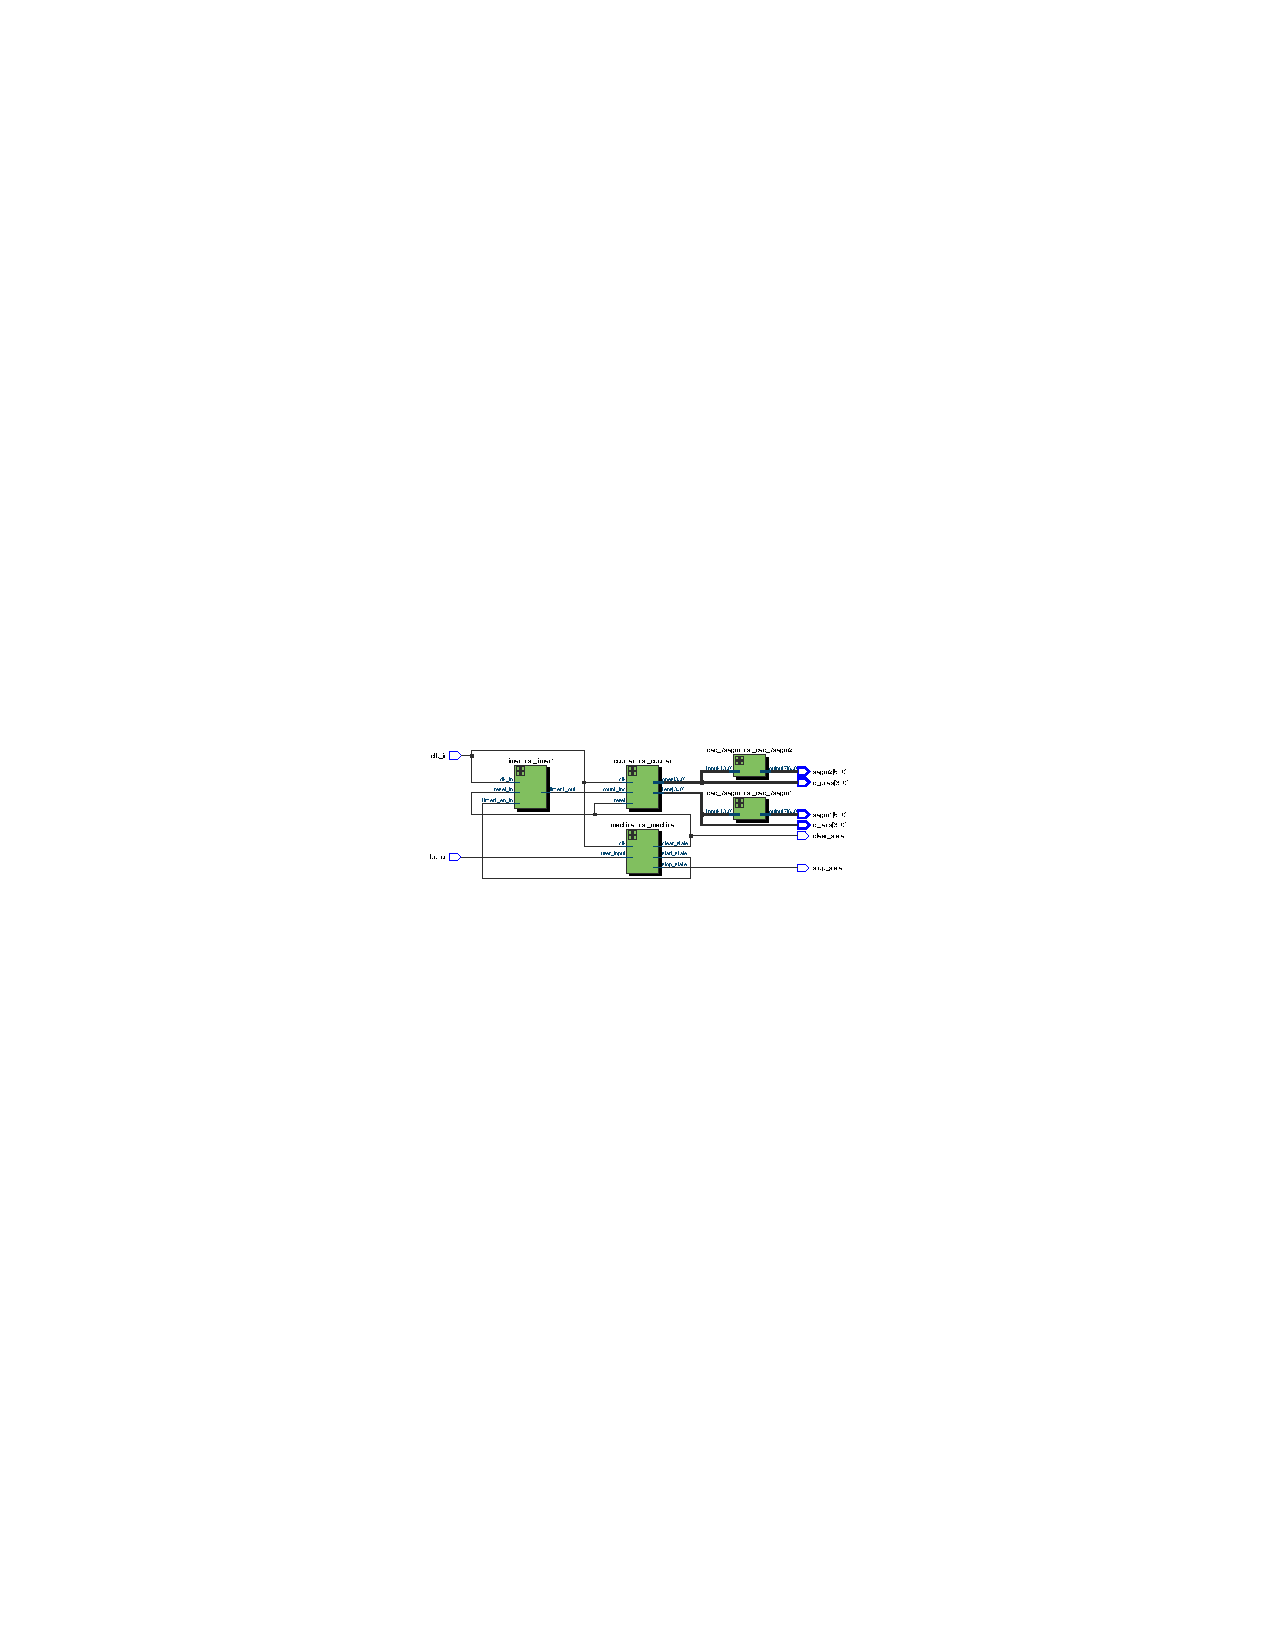
\includegraphics[clip,width=0.8\textwidth]{stopwatch.pdf}
	\end{figure}
	
	\section{Řídící stavový automat}
	Stavový automat byl navržen dle přiloženého obrázku. Je vytvořen tak, aby vstup byl ošetřen a nedocházelo k několika přechodům během 1 stisku tlačítka. Bylo tak zamezeno náhodnému přepínání. Při stavech \uv{s0} a \uv{s1} je aktivní výstup \uv{stop\_state}, při stavech \uv{s2} a \uv{s3} je aktivní výstup \uv{clear\_state} a pouze při stavu \uv{s4} je aktivní výstup \uv{start\_state} tak, aby okamžitě při stisku tlačítka pro zastavení opravdu došlo k zastavení a ne až po stisku.

	\begin{figure}[h]
		\centering
		\begin{tikzpicture}[scale=0.1]
			\tikzstyle{every node}+=[inner sep=0pt]
			\draw [black] (18.3,-18.4) circle (3);
			\draw (18.3,-18.4) node {$s0$};
			\draw [black] (33.7,-18.4) circle (3);
			\draw (33.7,-18.4) node {$s1$};
			\draw [black] (48.7,-18.4) circle (3);
			\draw (48.7,-18.4) node {$s2$};
			\draw [black] (48.7,-33.9) circle (3);
			\draw (48.7,-33.9) node {$s3$};
			\draw [black] (33.7,-33.9) circle (3);
			\draw (33.7,-33.9) node {$s4$};
			\draw [black] (18.3,-33.9) circle (3);
			\draw (18.3,-33.9) node {$s5$};
			\draw [black] (16.977,-15.72) arc (234:-54:2.25);
			\draw (18.3,-11.15) node [above] {$0$};
			\fill [black] (19.62,-15.72) -- (20.5,-15.37) -- (19.69,-14.78);
			\draw [black] (32.377,-15.72) arc (234:-54:2.25);
			\draw (33.7,-11.15) node [above] {$1$};
			\fill [black] (35.02,-15.72) -- (35.9,-15.37) -- (35.09,-14.78);
			\draw [black] (21.3,-18.4) -- (30.7,-18.4);
			\fill [black] (30.7,-18.4) -- (29.9,-17.9) -- (29.9,-18.9);
			\draw (26,-18.9) node [below] {$1$};
			\draw [black] (36.7,-18.4) -- (45.7,-18.4);
			\fill [black] (45.7,-18.4) -- (44.9,-17.9) -- (44.9,-18.9);
			\draw (41.2,-18.9) node [below] {$0$};
			\draw [black] (47.377,-15.72) arc (234:-54:2.25);
			\draw (48.7,-11.15) node [above] {$0$};
			\fill [black] (50.02,-15.72) -- (50.9,-15.37) -- (50.09,-14.78);
			\draw [black] (48.7,-21.4) -- (48.7,-30.9);
			\fill [black] (48.7,-30.9) -- (49.2,-30.1) -- (48.2,-30.1);
			\draw (48.2,-26.15) node [left] {$1$};
			\draw [black] (50.023,-36.58) arc (54:-234:2.25);
			\draw (48.7,-41.15) node [below] {$1$};
			\fill [black] (47.38,-36.58) -- (46.5,-36.93) -- (47.31,-37.52);
			\draw [black] (45.7,-33.9) -- (36.7,-33.9);
			\fill [black] (36.7,-33.9) -- (37.5,-34.4) -- (37.5,-33.4);
			\draw (41.2,-33.4) node [above] {$0$};
			\draw [black] (35.023,-36.58) arc (54:-234:2.25);
			\draw (33.7,-41.15) node [below] {$0$};
			\fill [black] (32.38,-36.58) -- (31.5,-36.93) -- (32.31,-37.52);
			\draw [black] (30.7,-33.9) -- (21.3,-33.9);
			\fill [black] (21.3,-33.9) -- (22.1,-34.4) -- (22.1,-33.4);
			\draw (26,-33.4) node [above] {$1$};
			\draw [black] (19.623,-36.58) arc (54:-234:2.25);
			\draw (18.3,-41.15) node [below] {$1$};
			\fill [black] (16.98,-36.58) -- (16.1,-36.93) -- (16.91,-37.52);
			\draw [black] (18.3,-30.9) -- (18.3,-21.4);
			\fill [black] (18.3,-21.4) -- (17.8,-22.2) -- (18.8,-22.2);
			\draw (18.8,-26.15) node [right] {$0$};
			\draw [black] (9.3,-18.4) -- (15.3,-18.4);
			\draw (8.8,-18.4) node [left] {$INPUT$};
			\fill [black] (15.3,-18.4) -- (14.5,-17.9) -- (14.5,-18.9);
			\end{tikzpicture}
	\end{figure}
	
	\section{Detekce délky stisknutí tlačítka}
	Detekce délky stisknutí tlačítka byla již obtížnější částí úlohy. Jako vstupy jsou v tomto bloku využity \uv{stop\_state} a \uv{clear\_state} z předchozího bloku pro korektní nulování a funkcionalitu. Dále je zde uživatelský vstup tlačítko 2. Při držení tlačítka 2 je spuštěn časovač a logická 1 je uložena v klopném obvodu D. Výstup časovače je vstupem detekčního stavového automatu. Hodnota detekčního automatu je následně uložena pomocí multiplexoru a klopného obvodu D. Výstupy jsou ošetřeny tak, aby nebyly aktivní během držení tlačítka. Krátký stisk je dále určen dlouhým stiskem a to tak, že pokud je dlouhý stisk nadetekován, tak nemůže být aktivní krátký stisk.
	
	\begin{figure}[h]
		\centering
		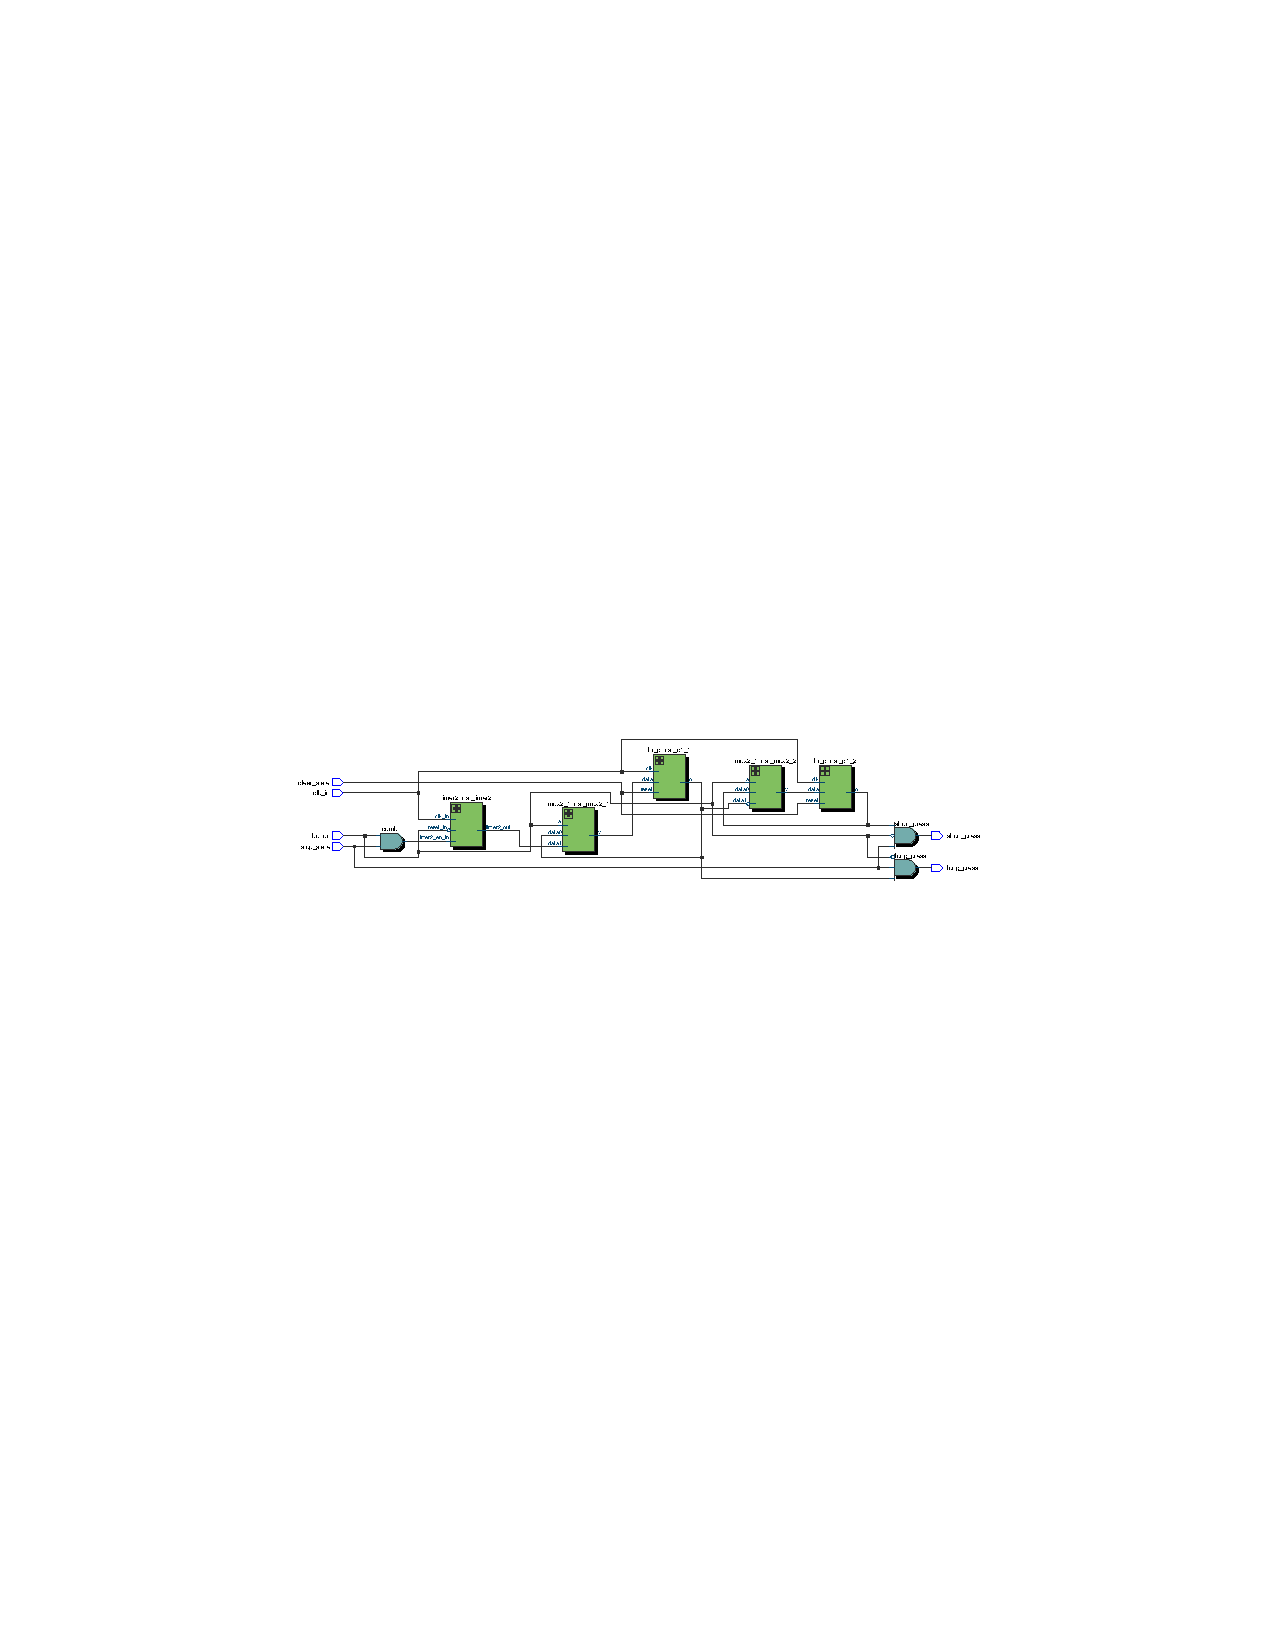
\includegraphics[clip,width=1\textwidth]{hold_detector.pdf}
	\end{figure}

	\section{Detekční stavový automat}
	Jedná se o velice jednoduchý automat, který má aktivní výstup pouze ve stavu \uv{s3}. Slouží pro detekci alespoň 2 pulzů ze vstupu. Zároveň je resetován při rozepnutí tlačítka 2, protože automat nemá jak se vrátit do počátečního stavu.

	\begin{figure}[h]
		\centering
		\begin{tikzpicture}[scale=0.1]
			\tikzstyle{every node}+=[inner sep=0pt]
			\draw [black] (20,-21.6) circle (3);
			\draw (20,-21.6) node {$s0$};
			\draw [black] (34.8,-21.6) circle (3);
			\draw (34.8,-21.6) node {$s1$};
			\draw [black] (34.8,-35.6) circle (3);
			\draw (34.8,-35.6) node {$s2$};
			\draw [black] (20,-35.6) circle (3);
			\draw (20,-35.6) node {$s3$};
			\draw [black] (10,-21.6) -- (17,-21.6);
			\draw (9.5,-21.6) node [left] {$INPUT$};
			\fill [black] (17,-21.6) -- (16.2,-21.1) -- (16.2,-22.1);
			\draw [black] (18.677,-18.92) arc (234:-54:2.25);
			\draw (20,-14.35) node [above] {$0$};
			\fill [black] (21.32,-18.92) -- (22.2,-18.57) -- (21.39,-17.98);
			\draw [black] (23,-21.6) -- (31.8,-21.6);
			\fill [black] (31.8,-21.6) -- (31,-21.1) -- (31,-22.1);
			\draw (27.4,-22.1) node [below] {$1$};
			\draw [black] (33.477,-18.92) arc (234:-54:2.25);
			\draw (34.8,-14.35) node [above] {$1$};
			\fill [black] (36.12,-18.92) -- (37,-18.57) -- (36.19,-17.98);
			\draw [black] (34.8,-24.6) -- (34.8,-32.6);
			\fill [black] (34.8,-32.6) -- (35.3,-31.8) -- (34.3,-31.8);
			\draw (34.3,-28.6) node [left] {$0$};
			\draw [black] (31.8,-35.6) -- (23,-35.6);
			\fill [black] (23,-35.6) -- (23.8,-36.1) -- (23.8,-35.1);
			\draw (27.4,-35.1) node [above] {$1$};
			\draw [black] (21.323,-38.28) arc (54:-234:2.25);
			\draw (20,-42.85) node [below] {$0,1$};
			\fill [black] (18.68,-38.28) -- (17.8,-38.63) -- (18.61,-39.22);
			\draw [black] (36.123,-38.28) arc (54:-234:2.25);
			\draw (34.8,-42.85) node [below] {$0$};
			\fill [black] (33.48,-38.28) -- (32.6,-38.63) -- (33.41,-39.22);
		\end{tikzpicture}
	\end{figure}
	
	\section{Uložení a zobrazení hodnoty}
	Tento blok má jako vstup nadetekovanou délku stisku tlačítka 2 a aktuální hodnotu čítače z prvního bloku, tj. bloku realizují pouze stopky. Hodnoty čítače jsou přivedeny do multiplexoru, který je přepínán zjištěnou délkou stisku. Hodnoty jsou následně uloženy pomocí klopných obvodů D. Obdobně to funguje v případě zobrazení uložené hodnoty, ta se pouze uloží do dalších klopných obvodů D. Jejich výstup je následně přiveden do dekodéru a poté do segmentovek pro zobrazení hodnoty.
	
	\begin{figure}[h]
		\centering
		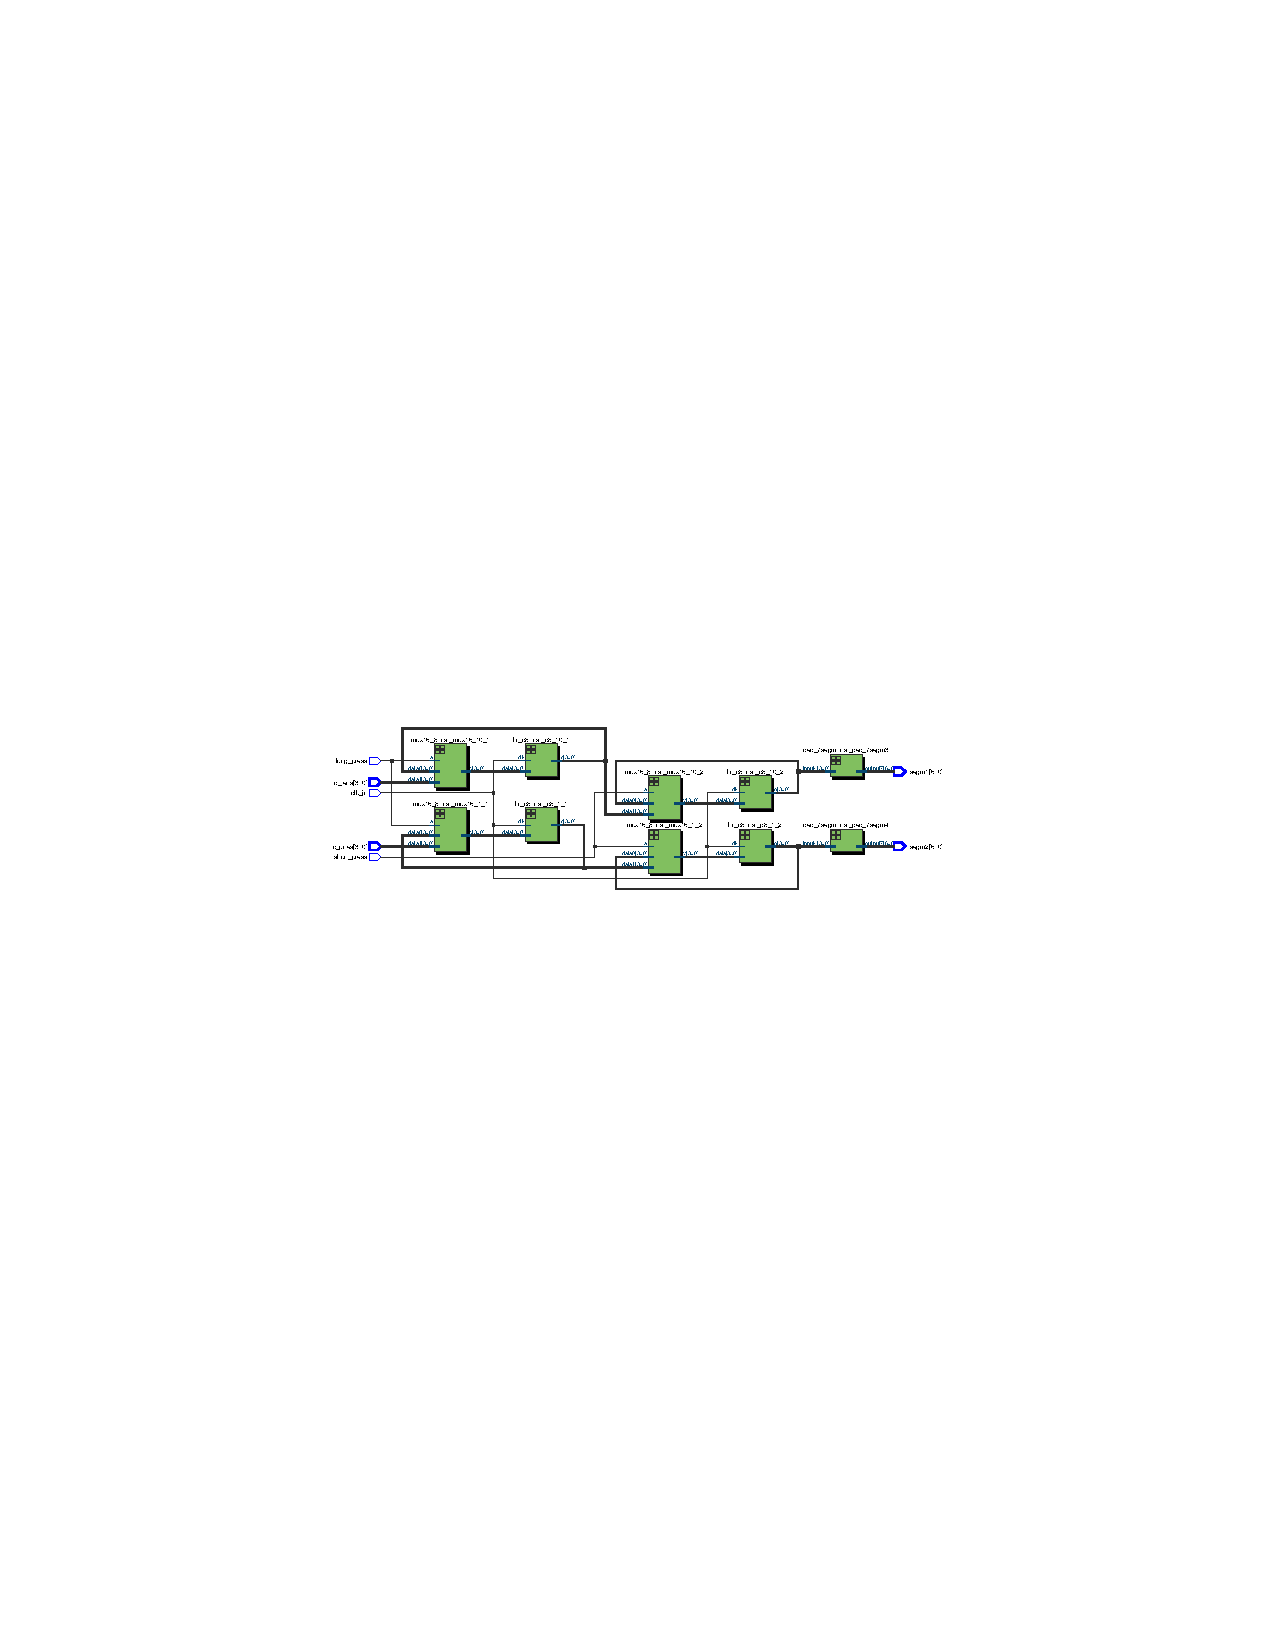
\includegraphics[clip,width=1\textwidth]{display_memory.pdf}
	\end{figure}
\end{document}